% mtron-graph.tex — the /a graph: uri path adjacency solid, uri→obj reference dotted
% The right-hand half of the side-by-side diagrams in docs/skills/mtron/SKILL.md.
% THIS FILE IS THE FIGURE'S SOURCE: the doc carries only the rendered PNG, so edit
% here, then re-render (standalone wrapper + \color{white}, then
% `pdftocairo -png -transp -r 300`) and drop the PNG in assets/mtron-graph.png.
%
% INK: the site theme is dark (--maincolor #000000, panels #191C24), so the body
% carries no colour and the render wrapper paints the ink white on a transparent
% page. Nothing here may set `fill`: a filled node would put an opaque patch
% behind a label.

% the mtron graph of /a — uri path adjacency solid, uri→obj reference dotted
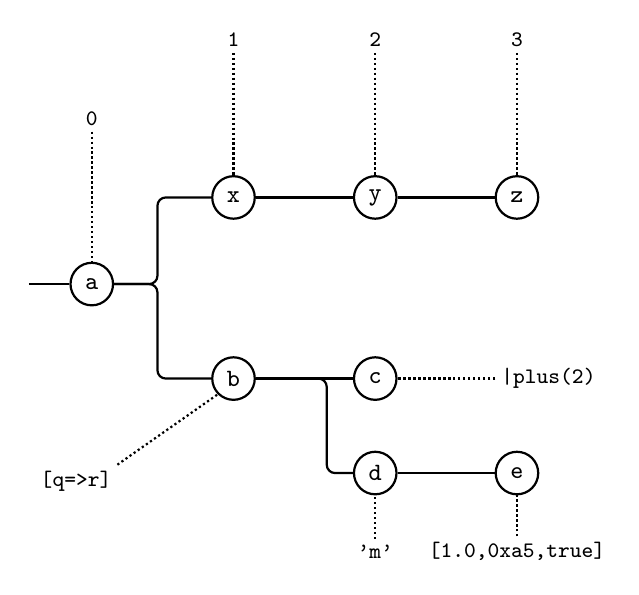
\begin{tikzpicture}[
  u/.style={font=\ttfamily\small, draw, circle, thick, minimum size=5.4mm, inner sep=0pt},  % a uri vertex (U)
  o/.style={font=\ttfamily\footnotesize, inner sep=2pt},                                    % its referent (O)
  p/.style={thick, rounded corners=3pt},                                                    % adjacency (solid)
  r/.style={densely dotted, thick},                                                         % reference (dotted)
]
% ── the uri path tree: one column per path segment
\node[u] (a) at (0,0)      {a};
\node[u] (x) at (1.8,1.1)  {x};
\node[u] (y) at (3.6,1.1)  {y};
\node[u] (z) at (5.4,1.1)  {z};
\node[u] (b) at (1.8,-1.2) {b};
\node[u] (c) at (3.6,-1.2) {c};
\node[u] (d) at (3.6,-2.4) {d};
\node[u] (e) at (5.4,-2.4) {e};

\draw[p] (-0.8,0) -- (a.west);                 % a is one segment of an enclosing path
\draw[p] (a.east) -- ++(0.55,0) |- (x.west);   % /a/x
\draw[p] (a.east) -- ++(0.55,0) |- (b.west);   % /a/b
\draw[p] (x.east) -- (y.west);                 % /a/x/y
\draw[p] (y.east) -- (z.west);                 % /a/x/y/z
\draw[p] (b.east) -- (c.west);                 % /a/b/c
\draw[p] (b.east) -- ++(0.9,0) |- (d.west);    % /a/b/d
\draw[p] (d.east) -- (e.west);                 % /a/b/d/e

% ── the referents, each hung off its uri by a dotted reference
\node[o] (o0) at (0,2.1)      {0};
\node[o] (o1) at (1.8,3.1)    {1};
\node[o] (o2) at (3.6,3.1)    {2};
\node[o] (o3) at (5.4,3.1)    {3};
\node[o] (rc) at (-0.2,-2.5)  {[q=>r]};
\node[o] (pl) at (5.8,-1.2)   {|plus(2)};
\node[o] (mm) at (3.6,-3.4)   {'m'};
\node[o] (ls) at (5.4,-3.4)   {[1.0,0xa5,true]};

\draw[r] (o0.south) -- (a.north);
\draw[r] (o1.south) -- (x.north);
\draw[r] (o2.south) -- (y.north);
\draw[r] (o3.south) -- (z.north);
\draw[r] (rc.north east) -- (b.south west);
\draw[r] (pl.west) -- (c.east);
\draw[r] (mm.north) -- (d.south);
\draw[r] (ls.north) -- (e.south);
\end{tikzpicture}
